\documentclass[11pt,a4paper]{article}
\usepackage[utf8]{inputenc}

\usepackage{geometry}
 \geometry{
 left=25mm,
 top=25mm,
 right=25mm,
 bottom=25mm,
 }
\usepackage{graphicx}	
\usepackage{bm}
\usepackage{url}
\usepackage{amsmath}	
\usepackage{tikz}
\usetikzlibrary{automata,arrows,positioning,calc}
\usepackage{todonotes}
%\renewcommand{\baselinestretch}{1.25}

\title{Decoding Performance of Convolutional Codes}
\author{Rasmus Vestergaard, Stefan Bejan and Daniel Pytlos}
\date{March 2017}

\begin{document}		
\maketitle

\todo[inline] {Compare different codes with the same constraint length but different (same number of) generator polynomials in both burst-error and random-error correction	.}

\todo[inline] {Compare different codes with the same constraint length and different code rate (more generator polynomials).}

This paper investigates the decoding performance of convolutional codes. This is done by simulating end-to-end transmission in different channels where messages are encoded using various convolutional codes.
Figure \ref{fig:simulationOverview} shows the logical setup of the simulation.

\begin{figure} [h]
\usetikzlibrary{shapes,arrows}

\tikzstyle{block} = [draw, rectangle, minimum height=3em, minimum width=6em]
\tikzstyle{input} = [coordinate]
\tikzstyle{output} = [coordinate]

\centering
\begin{tikzpicture}[auto, node distance=2cm,>=latex']
\centering

    % We start by placing the blocks
    \node [input, name=input] {};    
    \node [block, right of=input] (encoder) {Encoder};
    \node [block, right of=encoder, node distance=3cm] (channel){Channel};
    \node [block, right of=channel, node distance=3cm] (decoder){Decoder};
    \node [output, right of=decoder] (output) {}; 
    
    
    \draw [->] (encoder) -- node[name=u] {} (channel);
    \draw [->] (channel) -- node[name=v] {} (decoder);
    \draw [draw,->] (input) -- node {$\textbf{x}$} (encoder);
    \draw [->] (decoder) -- node [name=y] {$\hat{\textbf{x}}$}(output);

\end{tikzpicture}
\caption{\textit{Simulation overview} \label{fig:simulationOverview}}
\end{figure}

A message, $\textbf{x}$, consisting of $10^6$ bits is sent over a noisy channel. 2 types of channels are considered in this study:
\begin{itemize}\setlength\itemsep{0pt}
   \item Binary Symmetric Channel (BSC): Random, independant errors occur during transmission. The typical representation of a binary symmetric channel is shown in figure \ref{fig:bscChannel}
   \item Burst Error Channel: Errors are not independant, but occur in bursts.
\end{itemize}

\begin{figure} [b]
\centering
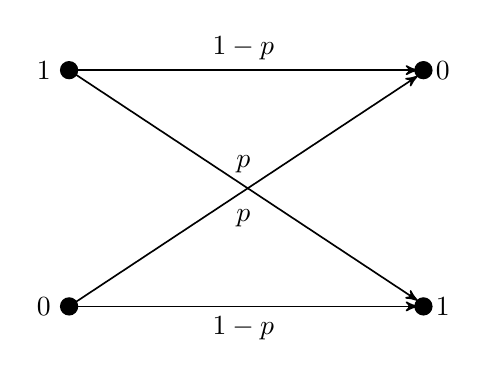
\begin{tikzpicture}[->, >=stealth', auto, semithick, node distance=3cm]
\centering
\filldraw (0,0) circle (3pt);
\filldraw (0,3) circle (3pt);
\filldraw (4.5,0) circle (3pt);
\filldraw (4.5,3) circle (3pt);
\draw[->,line width=0.6pt] (0,3) node[left=3pt] {$1$} -- node[above=1pt] {$p$} (4.425,0.075);
\draw[->,line width=0.6pt] (0,0) node[left=3pt] {$0$} -- node[below=3pt] {$p$} (4.425,2.925);
\draw[->,line width=0.6pt] (0,0) -- node[below] {$1-p$} (4.425,0.00)  node[right=3pt] {$1$};
\draw[->,line width=0.6pt] (0,3) -- node[above] {$1-p$} (4.425,3) node[right=3pt] {$0$};
\end{tikzpicture}
\caption{\textit{Binary Symmetric Channel}\label{fig:bscChannel}}
\end{figure}

The purpose of the study is to quantify the effects of different parameters of the convolutional code, namely the constraint length and the code rate. In order to achieve the best performance a trade-off analysis on the parameters needs to be performed. 
All simulations are conducted by utilizing MATLAB. Section \ref{sec:methodSection} presents the approach used to systematically determine the effect of code parameters in different channels. \todo{Analysis performed in sections 2-3-4}. Finally, section \ref{sec:conclusionSection} summarizes the findings.



\section{Method}
\label{sec:methodSection}

As a starting point for the analysis, the following 3 polynomial sets of convolutional codes were given. The first subscript represents the code number (further referenced in the report) and the second is the index of the generator polynomial associated with the code.

\begin{align*}
\begin{matrix}
Code 1&Code 2&Code 3\\
g_{1,1}(x) = 1 + x + x^2 + x^3 + x^6&g_{2,1}(x) = 1 + x^2 + x^3&g_{3,1}(x)=1 + x^2\\
g_{1,2}(x) = 1 + x^2 + x^3 + x^5 + x^6&g_{2,2}(x)=1 + x + x^3&g_{3,2} = 1+x+x^2\\
&g_{2,3}(x) = 1+x+x^2+x^3&g_{2,3}(x)=1+x+x^2\\
&&g_{3,4}(x) = 1+x+x^2
\end{matrix}
\end{align*}

We started our investigation by comparing how these given codes can handle random and burst errors on the channels. For this purpose, we designed 2 Matlab scripts that would allow us to simulate the transmission of a message over the given types of channels.

In both scripts, it is possible to adjust the input message length and the number of times the simulation should run. Increasing the number of simulation iterations will generates smoother lines of the figures, this reducing the stochastic effects on the results. For our simulations, we iterated the simulation 25 times, with different input messages.

A third file (\verb@trellisGenerator.m@), defining different convolutional code generator polynomials was required in order to easily change the code polynomials used to coding and decoding.

The scripts are summarized as follows:

\subsection{Random errors generation}

The file \verb@randomErrors.m@ presents the method of simulation of random errors on a BSC. In the script, it is possible to modify the following simulation parameters:

\begin{itemize}
   \item \verb@maxCER@ - maximum channel error rate. A value of 0.1 would mean that the channel can, at maximum, change 10\% of the transmitted bits.
   \item \verb@CERLevels@ - the number of different channel error levels for the simulation. This value determines the granularity of the increase steps for the error rate.  
\end{itemize}

For the specified number of iterations, the script generates a message of the given length. The message is then encoded using the code definitions from \verb@trellisGenerator.m@ file and for each of the codes, the encoded data is altered using the different levels of error probability. The alteration of bits at random positions in the message simulates the channel noise. For each of the error levels, the data is then decoded and compared to the transmitted version, calculating the Bit Error Rate (BER).

\subsection{Burst errors generation}

The file \verb@burstErrors.m@ presents the method of simulation of burst errors on a transmission channel. In the script, it is possible to modify the following simulation parameters:

\begin{itemize}
   \item \verb@BurstLevels@ - the number of different error burst lengths that are introduced on the channel. 
   \item \verb@nBursts@ - the total number of error bursts to be introduced on the channel.
   \item \verb@burstSep@ - the number of unaffected bits between error bursts.
\end{itemize}

Just as it happens in the case of the BSC, for the specified number of iterations, the script generates a message of the given length. The message is then encoded using the code definitions from \verb@trellisGenerator.m@ file and for each of the codes, the encoded data is altered using the different levels of burst error. The burst error represents a channel being temporarily affected by interference. For each level of burst, the data is then decoded and compared to the transmitted version, calculating the Burst Error (BE).
\\[8pt]

The results for the given codes are presented in section \ref{sec:givenCodesSection}. Even though the results, show as expected, a negative relation between the code rate and constraint length on one side and error rates on the other, we considered that simulations where we are varying only one of the factors are necessary. This approach allows us not only to confirm that both the factors influence the error correction capabilities of the code, but also to assess their sensibility.

In order to achieve the above mentioned, we needed to come up with 6 new set of codes namely Code 4 to 9. Their generator polynomials are presented below.

\begin{align*}
\begin{matrix}
Code 4&Code 5&Code 6\\
g_{4,1}(x) = 1 + x^2 + x^3&g_{5,1}(x) = 1 + x^2&g_{6,1}(x)=1 + x + x^2 + x^3 + x^6\\
g_{4,2}(x) = 1+x+x^2+x^3&g_{5,2}(x) = 1+x+x^2&g_{6,2}(x)=1 + x^2 + x^3 + x^5 + x^6\\
&&g_{6,3}(x)=1 + x + x^2 + x^3 + x^4 + x^5 + x^6\\
\end{matrix}\\
\begin{matrix}
Code 7&Code 8&Code 9\\
g_{7,1}(x) = 1 + x^2&g_{8,1}(x) = 1 + x + x^2 + x^3 + x^6&g_{9,1}(x)=1 + x^2 + x^3\\
g_{7,2}(x) = 1+x+x^2&g_{8,2}(x) = 1 + x + x^3 + x^4 + x^6&g_{9,2}(x)=1 + x + x^3\\
g_{7,3}(x) = 1+x+x^2&g_{8,3}(x) = 1 + x^2 + x^3 + x^5 + x^6&g_{9,3}(x)=1+x+x^2+x^3\\
&g_{8,4}(x) = 1 + x + x^2 + x^3 + x^4 + x^5 + x^6&g_{9,4}(x)=1+x+x^2+x^3\\
\end{matrix}
\end{align*}

Using the above mentioned codes, we were able to group them by code rate and by constraint length, as follows:

\begin{table}[h]
\centering
\caption{Grouping of codes based on code rate}
\begin{tabular}{ll}
\hline
Code rate &  Codes \\ \hline
1/2 & Code 1, Code 4, Code 5 \\
1/3 & Code 2, Code 6, Code 7 \\
1/4 & Code 3, Code 8, Code 9 \\
\end{tabular}
\end{table}

\begin{table}[h]
\centering
\caption{Grouping of codes based on constraint length}
\begin{tabular}{ll}
\hline
Constraint length &  Codes \\ \hline
3 & Code 3, Code 5, Code 7 \\
4 & Code 2, Code 4, Code 9 \\
7 & Code 1, Code 6, Code 8 \\
\end{tabular}
\end{table}

The results obtained when having the constant code rate of 1/2 and variable constraint length are presented in section \ref{sec:constantCodeRateSection}. Similarly, the results obtained by having a constant constraint length of 4 and variable code lengths are presented in section \ref{sec:constantContraintLengthSection}.

 
\subsection{Markov Burst Error Channels}
While the previous channels are easy to deal with in theory, in many cases it does not match the reality well. In practice, errors are neither entirely independant and random, nor deterministic bursts, but rather stochastic with correlation. Effects such as deep fades in wireless channels cause the probability of a symbol being in error to be much larger if the previous symbol was an error. This causes errors to appear in bursts. A simple model of such a channel can be created by using a two-state Markov chain, as shown on figure \ref{fig:markovChain}. For each time-step (each bit in the channel), the current state of the chain is updated and a bit is output. The transition probabilities $p_{01}$ and $p_{10}$ determines how the error pattern will behave. $p_{01}$ is the probability of starting a burst, and $p_{10}$ is the probability of ending the current burst. In this way, the length of bursts, BL, will be geometrically distributed:\todo{Can add a plot of this for chosen p10 if room for it.}
\begin{equation}
P(\text{BL} = k) = (1-p_{10})^{k-1}  p_{10}
\end{equation}
meaning that smaller bursts are more likely than long bursts. The Markov burst error channel will be simulated by basing the error pattern on this Markov chain.
\begin{figure}[t]
\centering
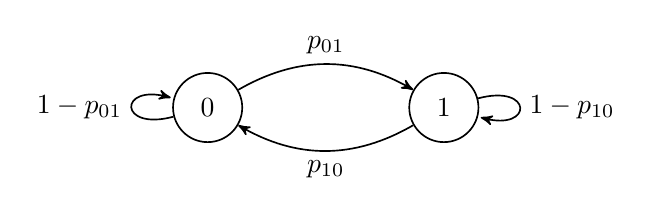
\begin{tikzpicture}[->, >=stealth', auto, semithick, node distance=3cm]
\centering
\node[state] (A) at (0,0) {$0$};
\node[state] (D) at (3,0) {$1$};
\path(A) edge[loop left] node{$1-p_{01}$} (A);
\path(A) edge[bend left] node{$p_{01}$} (D);
\path(D) edge[bend left] node{$p_{10}$} (A);
\path(D) edge[loop right] node{$1-p_{10}$} (D);
\end{tikzpicture}
\caption{\textit{Markov Chain for Burst Channel Simulation}\label{fig:markovChain}}
\end{figure}

The file \verb@markovErrors.m@ contains the implementation of this method for simulation of these random burst errors. It is possible to modify the following simulation parameters:
\begin{itemize}\setlength\itemsep{0pt}
\item \verb@burstProbabilityMax@, max value for $p_{01}$ to be simulated.
\item \verb@burstProbabilityLevels@, number of different levels of $p_{01}$ to be simulated. Determines the granularity of the simulation.
\item \verb@p10@, the transition probability from state $1$ to $0$
\end{itemize}
For each of the specified number of simulations, a message is generated and encoded using the code definitions from \verb@trellisGenerator.m@ and for each of these transmission through a number of Markov channels, where the transition parameter $p_{01}$ is varied according to the specified parameters, is simulated. The CER of each Markov channel is calculated. The received codeword is then decoded and compared to the real message. Finally, the BER is calculated.
\section{Given codes}
\label{sec:givenCodesSection}	
\input{givenCodes}


\section{Constant code rate}
\label{sec:constantCodeRateSection}

\begin{figure}
\centering
\includegraphics[scale=1]{../figures/randomErrors-crop.pdf} 
\caption{Decoding after BSC.\todo[inline]{May want to resize eventually.}}
\end{figure}



\section{Constant constraint length}
\label{sec:constantContraintLengthSection}

\begin{figure}
\centering
\includegraphics[scale=1]{../figures/extra12rand.pdf} 
\caption{1/2 rate\todo[inline]{change caption}}
\end{figure}

\begin{figure}
\centering
\includegraphics[scale=1]{../figures/extra12burst.pdf} 
\caption{1/2 rate\todo[inline]{change caption}}
\end{figure}

\begin{figure}
\centering
\includegraphics[scale=1]{../figures/extra12markov.pdf} 
\caption{1/2 rate\todo[inline]{change caption}}
\end{figure}

\todo[inline] {Create a markov burst-error channel?}

\section{Conclusion}
\label{sec:conclusionSection}



The simulations performed in sections \ref{sec:givenCodesSection}, \ref{sec:constantCodeRateSection} and \ref{sec:constantContraintLengthSection} show a number of features. As was expected, a decrease in code rate or an increase in constraint length in general will decrease the decoded BER. It was seen, however, that as the CER increases, eventually codes with high constraint rates will start to perform worse than codes with lower constraint rate. This means that if the channel is very poor, then increasing the constraint rate might actually have a negative effect on the decoded BER.
\\[6pt]
The code rate is seen to have a very big influence on the decoded BER in the BSC, and a smaller influence in the MBEC. This indicates that codes should be tailored to the specific channel in order to reach a target BER while maximizing throughput. If the probability of errors in the BSC is time-varying, techniques such as puncturing can be used to optimize the throughput, by increasing the code rate. To do this, feedback from the receiver about the current BER can be utilized. Then, when the BER is lower than the required BER, a puncturing matrix that gives a larger code rate can be used, increasing the throughput. The encoder and decoder must then continously coordinate how the puncturing is done to optimize the throughput with a constant BER.
\\[6pt]
In random burst error channels, such as the MBEC, as would likely be encountered in practice, it is less clear what to do. It was seen in figure \ref{fig:givenMarkovFigure}, that it is possible to achieve the same BER for two different codes, where one had code rate $1/3$ and one had code rate $1/2$. This indicates that the  throughput in burst error channels may be optimized by tailoring the constraint length to be long enough to handle the bursts in the channel. Simply increasing the constraint length is, however, not always a possibility, since the decoding complexity will increase. Therefore, other techniques such as interleaving with the depth tailored to the expected bursts in the channel could be used instead. It is hard to conclude much, except that in order to achieve optimum code rate for a given BER in such a channel, the used code must be specifically tailored to the channel.




\end{document}